\vorlesung{08. Februar 2018}

\chapter{Massive Neutrinos}
\begin{itemize}
\item[$\ra$] Im Standardmodell: $m_\nu = 0$
\item[$\ra$] Aus $\nu$-Oszillationen: $m_\nu >0$ (mindestens ein $m_\nu > 0.05$\,eV)
\item[$\ra$] Aus direkten Messungen: $m_\nu < 2$\,eV\\
(Kosmologie: $\sum m_\nu \lesssim 0.12$\,eV)
\end{itemize}
\section{Massen- und Flavoureigenzustände von Neutrinos}
Flavour: $\nu$-EZ der schwachen WW
\begin{align*}
\boxed{\nu_e, \ \nu_\mu, \ \nu_\tau}
\end{align*}
Masse: Eigenzustände der Propagation
\begin{align*}
\boxed{ \begin{matrix}
\nu_1, & \nu_2, & \nu_3\\
\ua & \ua & \ua\\
m_1, & m_2, & m_3
\end{matrix} }
\end{align*}
Oszillationen $\Ra$ $\lb  \nu_e, \ \nu_\mu, \ \nu_\tau\rb  \neq \lb \nu_1, \ \nu_2, \ \nu_3\rb $\\
$\Ra$ Mischungmatrix (ähnlich wie bei Quarks)
\begin{align}
\boxed{ \begin{pmatrix}
\nu_e \\ \nu_\mu \\ \nu_\tau 
\end{pmatrix} = U \lb 3\rb  \cdot \begin{pmatrix}
\nu_1 \\ \nu_2 \\ \nu_3
\end{pmatrix}}
\end{align}
Parameter: 3 Winkel, 1 komplexe Phase (Pontecorro-Maki-Nakagawa-Sakata-Matrix, PMNS)

Aus Oszillationen: Messung von 
\begin{align}
\Delta^2 m_{ij} = m_i^2 - m_j^2
\end{align}
$\lt$ 2 unabhängige Werte
\begin{align}
\labs \Delta m_{23}^2 \rabs \approx 2.4 \cdot 10^{-3}\,\mr{eV^2}\\
\Delta m_{13}^2 \approx 7.6\cdot 10^{-5}\,\mr{eV^2}\\
\Ra \text{ ein } m_i \geq \sqrt{\labs m_{23}^2 \rabs} \approx 0.05\,\mr{eV}
\end{align}
Achtung: $\nu_e, \ \nu_\mu,\ \nu_\tau$ haben \tb{keine} wohldefinierte Masse!\\
Experimentelle Grenzen auf:
\begin{align}
\lla m^2 \lb \nu_e\rb  \rra = \sum \labs U_{e,i} \rabs^2 m_i^2 \qquad (\beta\text{-Zerfall})\\
\lla m_{\beta\beta} \rra = \labs \sum U_{e,i}^2 m_i \rabs \qquad (0\nu 2\beta)\\
\lla m_\mr{kosm.} \rra = \sum m_i \qquad (\text{Kosmologie})
\end{align}
\section{Direkte Messung der Neutrinomasse}
Erinnerung an \ref{sec:5.2}:\\
Messung von $\lla m^2 \lb \nu_e\rb \rra$ aus $e^-$-Spektrum bei $\beta$-Zerfall
\begin{figure}[!ht]
\centering
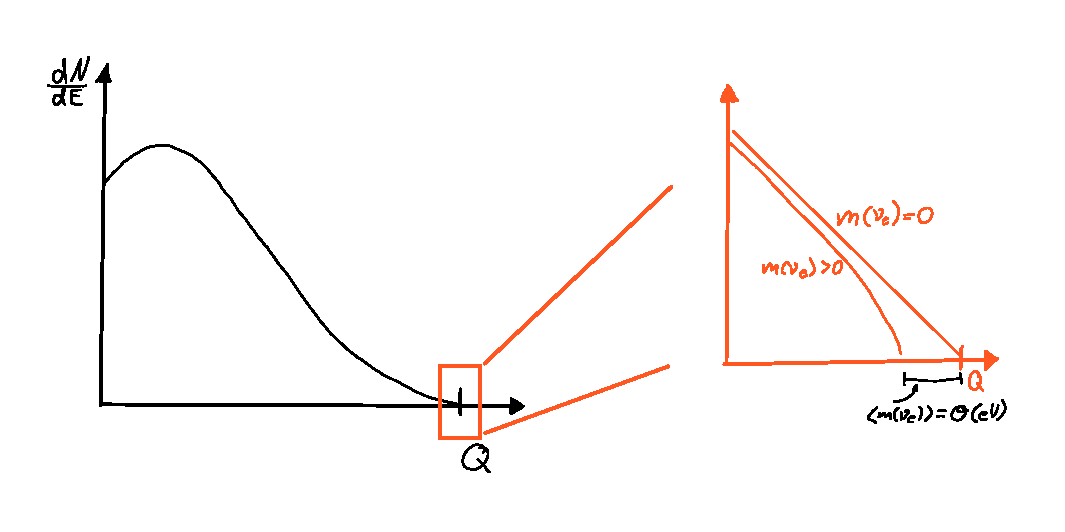
\includegraphics[width=.6\textwidth]{imgs/ep5-fig-9-1.pdf}
\captionof{figure}{Veränderung der Kurve aus Abb.\ref{fig:5.10} durch massebehaftete Neutrinos \label{fig:9.1}}
\end{figure}
\tb{Erforderlich:}
\begin{itemize}
\item Niedriger $Q$-Wert
\item $e^-$ werden ohne (stochstischen) Energieverlust freigesetzt
\item Hohe Zahl von Zerfällen
\item Extrem präzise Messung des Spektrums
\end{itemize}
Derzeit beste Lösung: Verwende Tritium-Zerfall
\begin{align}
\boxed{ ^3 H \ra ^3He + e^- + \bar{\nu}_e} \qquad Q = 18.6\,\mr{keV}
\end{align}
$\ra$ Spektrometer-MAC-E-Filter (magnetic adiabatic collimation, electrostatic)
\begin{figure}[!ht]
\centering
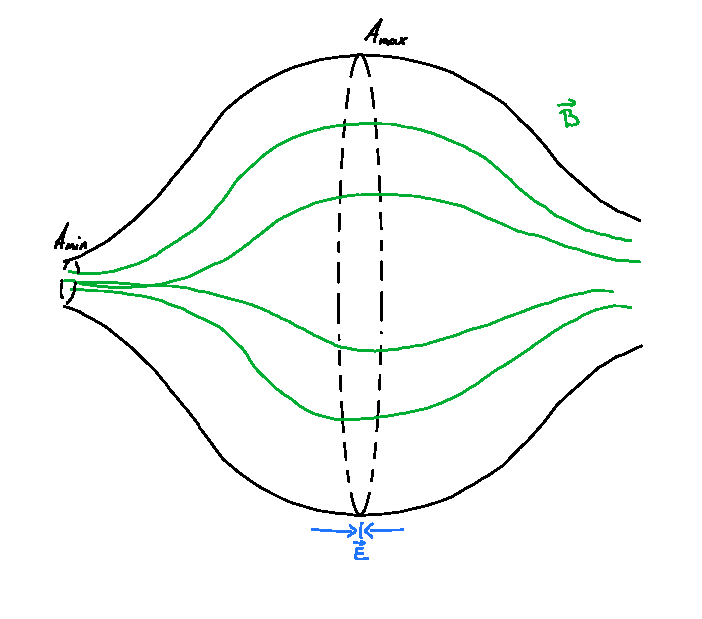
\includegraphics[width=.5\textwidth]{imgs/ep5-fig-9-2.pdf}
\captionof{figure}{Prinzip des MAC-E-Filters,  mit $\labs \vec{B}\rabs$ bei $A_\mr{min}$ im Bereich von Tesla\label{fig:9.2}}
\end{figure}
Die $e^-$ folgen den Feldlinien und alle solche $e^-$ mit $p_z >0$ werden \glqq eingefangen\grqq{}
\begin{align}
0 < E_\parallel = \frac{p_z^2}{2m_e} \leq Q
\end{align}
In der Mitte der Versuchsanordnung gilt $\labs \vec{B}\rabs$ klein:
\begin{align}
B_\mr{min} = \frac{A_\mr{min}}{A_\mr{max}} B_\mr{max}
\end{align}
Der $e^-$-Transport entlang $\vec{B}$ ist adiabatisch\\
$\Ra$ magnetisches Moent der Kreisbewegung um $\vec{B}$ erhalten\\
$e^-$-Beugung in Ebene $\perp\vec{B}$ erzeugt magnetisches Moment
\begin{align}
\mu = I \cdot a = \pi e \nu R^2
\end{align}
\begin{compactitem}
\item[mit] $I$: Strom $e \cdot \nu$
\item[] $\nu$: Umlauffrequenz
\item[] $a$: Fläche der Kreisbahn
\end{compactitem}
\begin{align}
F_L = F_Z \nonumber\\
e v_T B = \frac{m_e v_T^2}{R} = \frac{2E_T}{R}\\
\Ra \ \mu = \pi e\nu R^2 = \frac{E_T}{B} = const.\\
\Ra E_T \lb B_\mr{min}\rb  = \frac{B_\mr{min}}{B_\mr{max}} E_T \lb B_\mr{max}\rb  = \frac{A_\mr{min}}{A_\mr{max}} E_T \lb B_\mr{max}\rb \\
\text{mit } \Delta E = \frac{B_\mr{min}}{B_\mr{max}} \cdot Q \nonumber
\end{align}
$\Ra$ In Spektrometermitte sind alle $e^-$-Impulse $\parallel\vec{B}$\\
$\Ra$ Zähle $e^-$, die Gegenspannung $V = \frac{Q}{e} - \frac{\delta E}{e}$ überwinden.\\
$\delta E$ einstellbar von 0 bis einige eV.

Bisherige Ergebnisse verträglich mit $m_\nu = 0$. Obergrenze bisher:
\begin{align}
\boxed{ \lla m\lb \nu_e\rb \rra < 2\,\mr{eV} \ @ \ 95\,\% C.L. }
\end{align}
Zukunft: KATRIN-Experiment, Sensitivität 0.2\,eV

Achtung: Auch Einschränkung aus Kosmologie, $\lla m_\mr{kosm.} \rra \lesssim 0.12$\,eV\\
Aber: Modellabhängig
\newpage
\section{Neutrinooszillationen}
\begin{itemize}
\item \tb{Was ist das?}\\
Neutrino-Flavour wandelt sich \glqq im Flug\grqq{} um, \tb{keine} WW involviert
\begin{figure}[!ht]
\centering
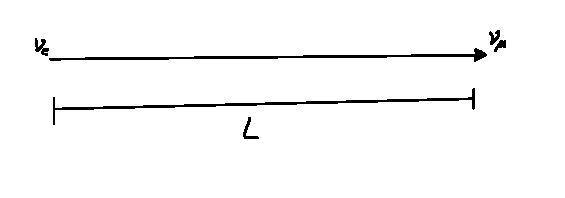
\includegraphics[width=.5\textwidth]{imgs/ep5-fig-9-3.pdf}
\captionof{figure}{Schematische Neutrinooszillation\label{fig:9.3}}
\end{figure}
\item Wie funktionieren sie?\\
\tb{Beispiel:} 2-Flavour-Mischung im Vakuum
\begin{align}
\binom{\nu_1}{\nu_2} = \begin{pmatrix}
\cos \theta & - \sin \theta \\ \sin \theta & \cos \theta
\end{pmatrix}\binom{\nu_e}{\nu_\mu}
\end{align}
(nicht relativistisch, aber gut zur Demonstration des Mechanismus)
\begin{itemize}
\item[$\ra$] $t=0$: Produktion eines $\nu_e$
\begin{align}
\Ra \ \ket{\nu \lb t=0\rb } = \ket{\nu_e} = \ket{\nu_1} \cdot \cos \theta + \ket{\nu_2} \cdot \sin \theta
\end{align}
\item[$\ra$] Propagation im Vakuum bis $t=T$
\begin{align}
\ket{\nu\lb t=T\rb } = \ket{\nu_1} \cdot \cos \theta \cdot e^{-iE_1t} + \ket{\nu_2} \sin \theta e^{-iE_2t}
\end{align}
Hierbei entwickelt sich jeder Zustand entsprechend seiner Masse
\item[$\ra$] Amplitude für $\lno \nu_e \rabs_{t=0} \ra \lno \nu_e\rabs_{t=T}$
\begin{align}
A_e = \braket{\nu_e | \nu\lb t=T\rb } = \cos^2 \theta e^{-iE_1t} + \sin^2 \theta e^{-iE_2t}\\
\braket{\nu_i|\nu_j} = \delta_{ij} \nonumber
\end{align}
\item[$\ra$] Wahrscheinlichkeit für $\nu_e \ra \nu_e$:
\begin{align}\begin{split}
P_e \labs A\rabs^2 = A_e \cdot A_e^*\\
P_e = \cos^4 \theta + \sin^4 \theta + \sin^2\theta \cos^2 \theta \underbrace{\lsb  e^{-i\lb E_1-E_2\rb t} + e^{i\lb E_1-E_2\rb t} \rsb }_{2 \cos \lb \Delta E \cdot t\rb }\\
= 1- 2 \sin^2 \theta \cos^2 \theta \lsb 1- \cos \lb \Delta E \cdot t\rb \rsb 
\end{split}\end{align}
Im Folgenden wird in Näherung davon ausgegangen, dass die Impulse identisch sind
\begin{align}
\begin{split}
\Delta E &= \sqrt{p^2+m_1} - \sqrt{p^2 +m_2^2}\\
& = p\lsb  1+ \frac 12 \frac{m_1^2}{p^2} -1- \frac 12 \frac{m_2^2}{p^2}\rsb \\
& = \frac{m_1^2 -m_2^2}{2p} = \frac{\Delta m^2}{2p}
\end{split}
\end{align}
weiterhin gilt für die Näherungen $v_\nu\approx c$, $t=\frac{L}{\mr{c}}$ und $p=E$, dass
\begin{align}
\begin{split}
1- \cos \lb \Delta E \cdot t\rb  = 2 \sin^2 \lb \frac{\Delta E \cdot t}{2}\rb  = 2 \sin^2 \lb  \frac{\Delta m^2 \cdot t}{4p}\rb = 2 \sin^2 \lb \frac{\Delta m^2 \cdot L}{4E}\rb 
\end{split}
\end{align}
und es ist
\begin{align}
2 \sin^2 \theta \cos^2 \theta = \frac 12 \sin^2 \lb 2 \theta\rb \nonumber \\
\boxed{P_e = 1- \sin^2 \lb 2 \theta \rb  \sin^2 \lb  \frac{\Delta m^2 L}{4E}\rb }
\end{align}
\item[$\Ra$] Oszillation nur, wenn $\theta \neq 0$ \tb{und} $\Delta m^2 \neq 0$ !
\item[$\ra$] Oszillationslänge:
\begin{align}
L_0 = \frac{\pi}{\nicefrac{\Delta m^2}{4E}} = 2.48 \, \mr{\frac{\nicefrac{E}{MeV}}{\nicefrac{\Delta m^2}{eV^2}}\cdot m}
\end{align}
\end{itemize}
\item Woher wissen wir, dass es $\nu$-Oszillationen gibt?
\begin{enumerate}
\item Sonnenneutrinos

In Sonne: Kernfusion, dominater Zyklus:
\begin{align}
\begin{split}
2e^- + 4p \ra ^4\mr{He} + 2 \nu_e + 26.73\,\mr{MeV}\\
2\lla E_\nu\rra = 0.59\,\mr{MeV}
\end{split}
\end{align}
Diese Energie entspricht ungefähr 2\,\% der elmag Energie.

Neutrinofluss auf der Erde:
\begin{align*}
\Phi_{\nu_e} = 2\cdot \frac{S}{26.73\,\mr{MeV}} = 6.5\cdot 10^{10} \, \mr{cm^{-2}\cdots^{-1}}\\
S = 8.5\times 10^{11}\,\mr{\nicefrac{MeV}{cm^2s}}
\end{align*}
\begin{compactitem}
\item[mit] $S$: Solarkonstante = Strahlungsleistung der Sonne auf der Erde
\end{compactitem}
Zusätzlich: $\nu$'s von Fusionsreaktionen schwerer Kerne $\ra$ $E$-Spektrum bis $\sim\ 20\,\mr{MeV}$.

\tb{Nachweis:}
\begin{itemize}
\item[$\ra$] Radiochemische Experimente\\
Homestake (1970-94): $\nu_e +^{37}U \ra e^- + ^{37}Ag$\\
GALLEX, SAGE ('90er): $\nu_e + ^{71}Ga \ra e^- + ^{71}Ge$\\
chemische Extraktion, Nachweis über Zerfall
\item[$\ra$] Direkt\\
Kamiokanne (1985-95) und Super-Kamiokanne (1996- : $\nu_ee^- \ra \nu_ee^-$)\\
SNO (1999-2006) $\nu_ed \ra e^-pp$, $\nu_xd \ra np$

Ergebnisse:
\begin{itemize}
\item[$\lt$] weniger $\nu_e$ als von Sonnenmodell erwartet in allen Experimenten
\end{itemize}
Aber: SNO-Experiment findet erwartete $\nu$-Fluss in $\nu_e + \nu_\mu+\nu_\tau$
\begin{itemize}
\item[$\Ra$] $\boxed{\text{Oszillation } \nu_e \ra \nu_{\cancel{e}}}$
\end{itemize}
\end{itemize}
\item Atmosphärische Neutrinos

Werden in Reaktionen kosmischer Strahlung mit Atomkernen der Atmosphäre gebildet
\begin{align}
\begin{split}
(p \text{ oder } A) +A \ra \pi^\pm \pi \pi \dots\\
\pi^\pm \ra \mu^\pm + \nu_e \text{ oder } \bar{\nu}_e\\
\mu^\pm \ra e^\pm + (\nu_e + \nu_\mu \text{ oder } \bar{\nu}_e + \bar{\nu}_\mu)
\end{split}
\end{align}
Damit wird ein Verhältnis erwartet:
\begin{align}
\Ra \frac{\nu_\mu + \bar{\nu}_\mu}{\nu_e + \bar{\nu}_e} \approx 2
\end{align}
\begin{itemize}
\item[$\ra$] Gemessen:
\begin{itemize}
\item[$\ra$] $\nu_\mu$ \glqq von unten\grqq{} fehlen
\item[$\ra$] kein Überschuss an $\nu_e$
\item[$\Ra$] $\boxed{\text{Übergang } \nu_\mu \ra \nu_\tau}$
\end{itemize}
\end{itemize}
\item Reaktor-Neutrinos

Stammen aus Kernspaltung, d.h. Umwandlungen $n\ra p$
\begin{align}
\boxed{n \ra p + e^- + \bar{\nu}_e}
\end{align}
Mit $E_{\bar{\nu}_e}\approx \mc{O}\lb 1\,\mr{MeV}\rb $

\tb{Nachweis} über $\bar{\nu}_e + p \ra e^+ + n$\\
Experimente u.a. KAMLAND (Japan), Daya Bay (China), Double Chooz (Belgien)\\
Information zu: Übergänge $\nu_e \ra \nu_e$
\end{enumerate}
\item \tb{Stand der Messungen}
\begin{align}
\Delta m_{12}^2 = 7.4\times 10^{-5}\,\mr{eV^2}\\
\labs \Delta m_{23}^2\rabs \approx 2.5\times 10^{-3}\,\mr{eV^2}\\
\lno \begin{matrix}
\sin^2 \theta_{12} \approx 0.297\\ \sin^2 \theta_{13} \approx 0.021 \\ \sin^2 \theta_{23} \approx 0.5
\end{matrix}\rrb \text{ PMNS-Matrix nicht diagonal-dominant}
\end{align}
Noch unbekannt:
\begin{itemize}
\item[$\lt$] Vorzeichen von $\Delta m_{23}^2$
\item[$\lt$] komplexe Phase
\item[$\lt$] absoluter Wert von $m_1$, $m_2$, $m_3$
\end{itemize}
\newpage

\item \tb{Neutrinooszillation in Materie}

zusätzliche Feynman-Graphen für $\nu_e$, $\bar{\nu}_e$
\begin{figure}[!ht]
\centering
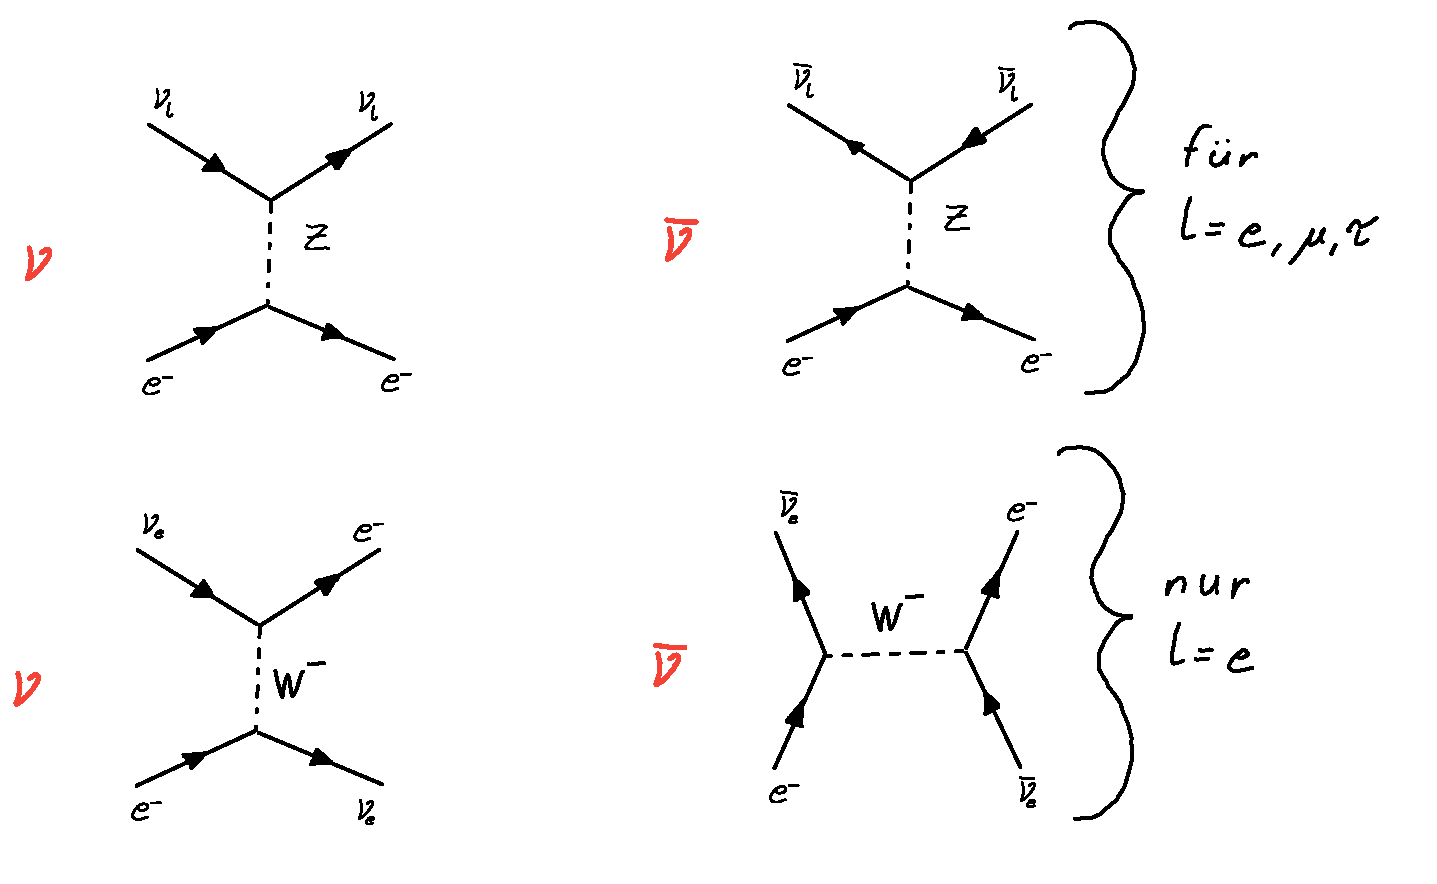
\includegraphics[width=.8\textwidth]{imgs/ep5-fig-9-4.pdf}
\caption{Feynmandiagramm für die Oszillation in Materie, wobei für Elektronen-(Anti-)Neutrinos auch unter Austausch eines $W^-$-Bosons wechselwirken können.}
\end{figure}
\begin{itemize}
\item[$\Ra$] unterschiedliche Amplitude für Vorwärtsstreuung
\item[$\ra$] unterschiedlicher Brechungsindex
\item[$\ra$] modifiziert $\nu$-Oszillation
\item[$\ra$] Entscheidend für Oszillationen von Sonnenneutrinos
\end{itemize}
\end{itemize}
